% LearningToOptimize.jl / L2OCore: how an optimization proxy is trained and used.
%
% A parametric problem (T1) is sampled through its parameters p; a proxy phi_theta
% maps p to a raw output z; the method turns z into a training loss, or, at
% inference, completes it into a prediction (x-hat, y-hat). Repair layers are
% optional wrappers: BoundedOutput (T6) before the loss and the completion,
% ProjectionRepair (T7) at inference only. Notation follows docs/src/theory.md.
%
% Build: make -C docs/src/assets/diagrams/src
%   pdflatex -jobname=learningtooptimize--method method.tex          -> wide layout
%   pdflatex -jobname=learningtooptimize--method-compact method.tex  -> narrow layout
\documentclass[tikz,border=4pt]{standalone}
% Shared style of the LearningToOptimize diagrams: the palette, lane frames, cards,
% chips and glyphs of the paper-style TikZ figures (the same visual system as the
% PortfolioOpt.jl and DecisionRules.jl figures). Each figure \input's this file.
\usepackage{amsmath,amssymb,bm}
\usepackage[T1]{fontenc}
\usepackage[scaled=0.92]{helvet}
\renewcommand{\familydefault}{\sfdefault}
\usetikzlibrary{arrows.meta,shapes.geometric,shapes.symbols,calc,positioning,decorations.pathreplacing}

\definecolor{dTeal}{HTML}{1A9AA0}
\definecolor{dTealLine}{HTML}{3FB3B8}
\definecolor{dNavy}{HTML}{3F4C8C}
\definecolor{dInk}{HTML}{1E2235}
\definecolor{dRed}{HTML}{E4573D}
\definecolor{dCoral}{HTML}{E2765A}
\definecolor{dOrange}{HTML}{F4A93B}
\definecolor{dPeach}{HTML}{FBD9AC}
\definecolor{dPanel}{HTML}{EEF0F2}
\definecolor{dGray}{HTML}{8A90A0}
\definecolor{dNode}{HTML}{14A3A8}
\definecolor{dShadow}{HTML}{D5DAE3}

% \ifcompact is true when the job name ends in "-compact" (narrow layout).
\newif\ifcompact
\ifnum\pdfmatch{-compact$}{\jobname}=1 \compacttrue\fi

\tikzset{
  >={Stealth[length=5pt,width=4pt]},
  every node/.style={text=dInk},
  title/.style={anchor=west,font=\small,inner sep=0pt},
  head/.style={font=\small\bfseries,text=dNavy},
  note/.style={font=\itshape\footnotesize,text=dNavy},
  dnote/.style={font=\itshape\footnotesize,text=dCoral},
  code/.style={font=\ttfamily\footnotesize,text=dNavy},
  store/.style={cylinder,shape border rotate=90,aspect=0.28,fill=dPeach,draw=dOrange,
                line width=0.7pt,minimum width=0.95cm,minimum height=1.2cm,font=\normalsize},
  dia/.style={diamond,fill=dOrange,draw=none,minimum size=0.9cm,inner sep=0pt,aspect=1,
              font=\normalsize},
  lnode/.style={circle,fill=dRed,draw=none,minimum size=0.66cm,inner sep=1pt,
                text=white,font=\normalsize},
  card/.style={rectangle,rounded corners=4pt,fill=white,draw=dShadow,line width=0.6pt},
  sheet/.style={rectangle,rounded corners=3pt,fill=dPanel,draw=dShadow,line width=0.6pt},
  chip/.style={rectangle,rounded corners=3pt,fill=dPanel,draw=none,font=\small,
               inner xsep=4pt,inner ysep=3pt},
  ochip/.style={chip,fill=white,draw=dGray,dashed,line width=0.6pt},
  pchip/.style={chip,fill=white,draw=dGray!70,dashed,line width=0.5pt,text=dGray},
  fwd/.style={->,dTealLine,line width=0.8pt},
  tgt/.style={->,dOrange,line width=0.9pt},
  dual/.style={->,dCoral,dashed,line width=0.9pt},
  dep/.style={->,dTealLine,line width=0.8pt},
  pdep/.style={->,dGray,dashed,line width=0.7pt},
  nn/.style={circle,minimum size=0.26cm,inner sep=0pt,draw=dInk!70,line width=0.35pt},
}

% Lane frame in the paper style: two shadow copies behind a teal rounded frame.
\newcommand{\lane}[4]{% #1 x0, #2 y0, #3 x1, #4 y1
  \foreach \o/\c in {0.16/dShadow!60,0.08/dShadow}
    \draw[\c,fill=white,rounded corners=5pt,line width=0.6pt]
      (#1+\o,#2-\o) rectangle (#3+\o,#4-\o);
  \draw[dTealLine,fill=white,rounded corners=5pt,line width=0.9pt] (#1,#2) rectangle (#3,#4);}

% Plain card frame (no shadow copies), for problems and losses.
\newcommand{\cardbox}[4]{\draw[dShadow,fill=white,rounded corners=4pt,line width=0.6pt] (#1,#2) rectangle (#3,#4);}

% Network glyph on one sheet. #1 = centre, #2 = name prefix, #3 = number of stacked
% sheets behind (0, 1 or 2).
\newcommand{\net}[3]{%
  \begin{scope}[shift={(#1)}]
    \ifnum#3>1 \node[sheet,minimum width=1.9cm,minimum height=1.8cm] at (0.30,0.22) {};\fi
    \ifnum#3>0 \node[sheet,minimum width=1.9cm,minimum height=1.8cm] at (0.15,0.11) {};\fi
    \node[sheet,minimum width=1.9cm,minimum height=1.8cm,fill=white] (#2sheet) at (0,0) {};
    \foreach \y [count=\i] in {0.36,0,-0.36} \node[nn,fill=dGray!45] (#2in\i) at (-0.64,\y) {};
    \foreach \y [count=\i] in {0.58,0.29,0,-0.29,-0.58} \node[nn,fill=dNode] (#2ha\i) at (-0.21,\y) {};
    \foreach \y [count=\i] in {0.44,0.15,-0.15,-0.44} \node[nn,fill=dNode] (#2hb\i) at (0.21,\y) {};
    \node[nn,fill=dOrange] (#2out) at (0.64,0) {};
    \foreach \a in {1,...,3} \foreach \b in {1,...,5} \draw[dGray!60,line width=0.2pt] (#2in\a) -- (#2ha\b);
    \foreach \a in {1,...,5} \foreach \b in {1,...,4} \draw[dGray!60,line width=0.2pt] (#2ha\a) -- (#2hb\b);
    \foreach \a in {1,...,4} \draw[dGray!60,line width=0.2pt] (#2hb\a) -- (#2out);
  \end{scope}}

% Jacobian mask glyph: an n x d grid with a few entries selected. #1 = centre.
\newcommand{\maskgrid}[1]{%
  \begin{scope}[shift={(#1)}]
    \foreach \i in {0,...,4} \foreach \j in {0,...,3}
      \draw[dShadow,fill=white,line width=0.4pt] (\j*0.2-0.4,-\i*0.2+0.5) rectangle ++(0.2,-0.2);
    \foreach \i/\j in {0/1,1/3,2/0,3/2,4/1}
      \draw[dOrange,fill=dOrange,line width=0.4pt] (\j*0.2-0.4,-\i*0.2+0.5) rectangle ++(0.2,-0.2);
  \end{scope}}

% Code names inside italic notes stay upright.
\newcommand{\cmd}[1]{{\upshape\ttfamily #1}}

% Software-architecture helpers: package cards, type chips and chip rows.
\tikzset{
  pkg/.style={rectangle,rounded corners=4pt,fill=white,draw=dShadow,line width=0.6pt,
              align=center,inner xsep=5pt,inner ysep=4pt,font=\footnotesize},
  pkgcore/.style={pkg,draw=dTealLine,line width=0.9pt},
  pkgplan/.style={pkg,draw=dGray,dashed,text=dGray},
  tchip/.style={chip,font=\ttfamily\footnotesize,inner xsep=3pt,inner ysep=2.5pt},
  tplan/.style={tchip,fill=white,draw=dGray,dashed,line width=0.5pt,text=dGray},
  absname/.style={anchor=west,font=\ttfamily\footnotesize,text=dNavy,inner sep=1pt},
}
% \chiprow{x}{y}{style}{A,B,C}: chips left to right from (x,y), anchored west.
\newcommand{\chiprow}[4]{%
  \coordinate (cr@next) at (#1,#2);
  \foreach \t in {#4} {%
    \node[#3,anchor=west] (cr@last) at (cr@next) {\t};
    \coordinate (cr@next) at ($(cr@last.east)+(0.12,0)$);}}


\newcommand{\problem}{%
  $\begin{aligned}
    \mathrm{OPT}(p)=\;&\min_{x}\;\; f(x;p)\\[1pt]
    &\;\text{s.t.}\;\; g_i(x;p)\in\mathcal{S}_i\;\;\forall i
  \end{aligned}$}

\begin{document}
\ifcompact
% ============================ narrow (phone) layout ============================
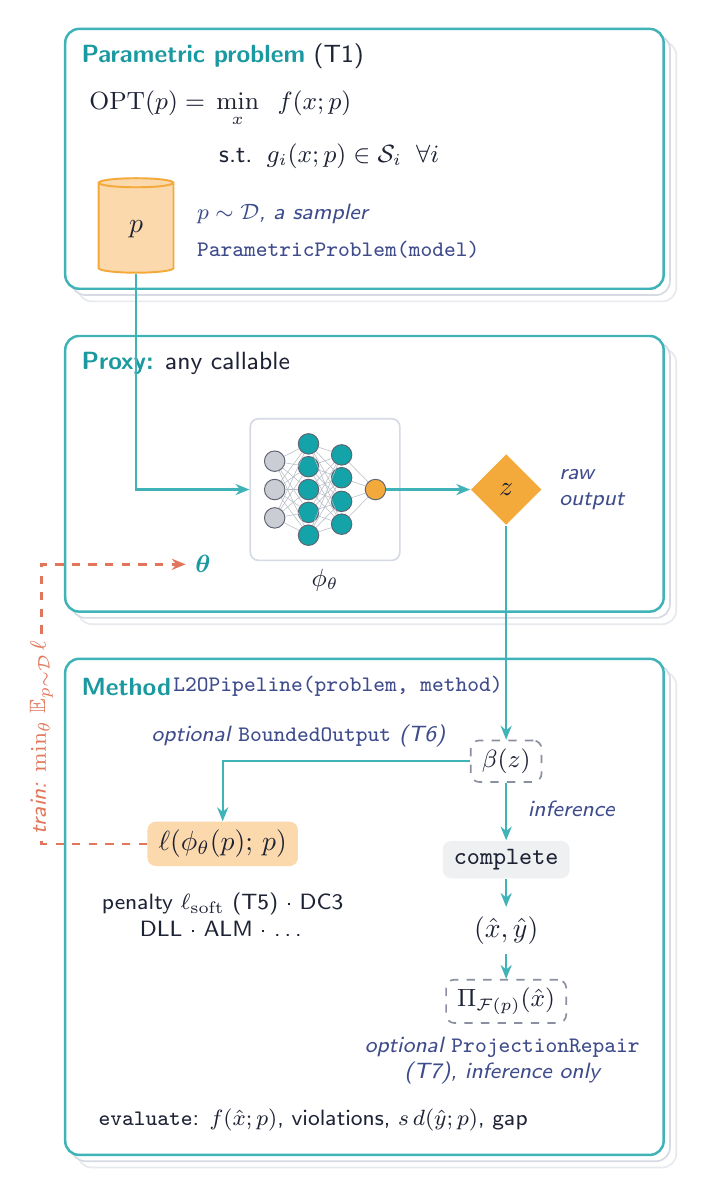
\begin{tikzpicture}
  % ---- parametric problem ----
  \lane{0}{11.0}{7.6}{14.3}
  \node[title] at (0.2,13.95) {\textcolor{dTeal}{\bfseries Parametric problem} (T1)};
  \node[anchor=north west,font=\small,inner sep=0pt] at (0.3,13.55) {\problem};
  \node[store] (p) at (0.9,11.75) {$p$};
  \node[note,anchor=west] at (1.55,11.95) {$p\sim\mathcal{D}$, a sampler};
  \node[code,anchor=west] at (1.55,11.5) {ParametricProblem(model)};
  % ---- proxy ----
  \lane{0}{6.9}{7.6}{10.4}
  \node[title] at (0.2,10.05) {\textcolor{dTeal}{\bfseries Proxy:} any callable};
  \net{3.3,8.45}{px}{0}
  \node[font=\small\bfseries,text=dTeal] (th) at (1.75,7.5) {$\bm\theta$};
  \node[font=\small] at (3.3,7.3) {$\phi_\theta$};
  \node[dia] (z) at (5.6,8.45) {$z$};
  \node[note,anchor=west,align=left] at (6.15,8.45) {raw\\output};
  \draw[fwd] (pxout.east) -- (z.west);
  \draw[fwd] (p.south) -- (0.9,8.45) -- (pxsheet.west);
  % ---- method ----
  \lane{0}{0}{7.6}{6.3}
  \node[title] at (0.2,5.95) {\textcolor{dTeal}{\bfseries Method}};
  \node[code,anchor=west] at (1.25,5.95) {L2OPipeline(problem, method)};
  \node[ochip] (bo) at (5.6,5.0) {$\beta(z)$};
  \draw[fwd] (z.south) -- (bo.north);
  \node[note,anchor=south east] at (4.95,5.05) {optional \cmd{BoundedOutput} (T6)};
  % training branch
  \node[chip,font=\normalsize,fill=dPeach] (loss) at (2.0,3.95) {$\ell(\phi_\theta(p);\,p)$};
  \draw[fwd] (bo.west) -| (loss.north);
  \node[font=\footnotesize,align=center] at (2.0,3.05) {penalty $\ell_{\mathrm{soft}}$ (T5) · DC3\\DLL · ALM · \dots};
  % inference branch
  \node[chip] (comp) at (5.6,3.75) {\texttt{complete}};
  \node (xy) at (5.6,2.85) {$(\hat x,\hat y)$};
  \node[ochip] (pr) at (5.6,1.95) {$\Pi_{\mathcal{F}(p)}(\hat x)$};
  \node[note,align=center] at (5.55,1.2) {optional \cmd{ProjectionRepair}\\(T7), inference only};
  \draw[fwd] (bo.south) -- (comp.north);
  \node[note,anchor=west] at (5.75,4.4) {inference};
  \draw[fwd] (comp.south) -- (xy.north);
  \draw[fwd] (xy.south) -- (pr.north);
  \node[font=\footnotesize,anchor=west] at (0.3,0.45) {\texttt{evaluate}: $f(\hat x;p)$, violations, $s\,d(\hat y;p)$, gap};
  % ---- training return ----
  \draw[dual] (loss.west) -- (-0.3,3.95) -- (-0.3,7.5) -- (th.west);
  \node[dnote,rotate=90,fill=white,inner sep=1pt] at (-0.3,5.3) {train: $\min_\theta\,\mathbb{E}_{p\sim\mathcal D}\,\ell$};
\end{tikzpicture}
\else
% =============================== wide layout ===================================
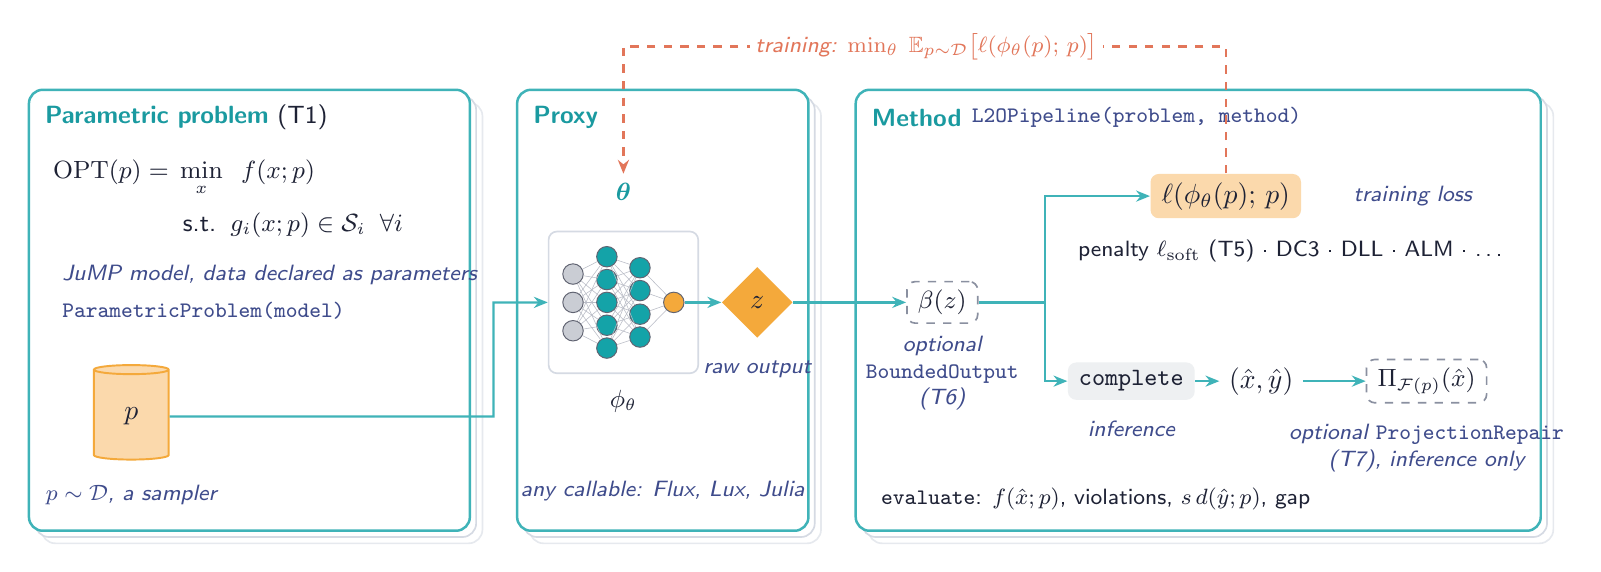
\begin{tikzpicture}
  % ---- parametric problem ----
  \lane{0}{0}{5.6}{5.6}
  \node[title] at (0.2,5.25) {\textcolor{dTeal}{\bfseries Parametric problem} (T1)};
  \node[anchor=north west,font=\small,inner sep=0pt] at (0.3,4.75) {\problem};
  \node[note,anchor=west] at (0.3,3.25) {JuMP model, data declared as parameters};
  \node[code,anchor=west] at (0.3,2.8) {ParametricProblem(model)};
  \node[store] (p) at (1.3,1.45) {$p$};
  \node[note] at (1.3,0.45) {$p\sim\mathcal{D}$, a sampler};

  % ---- proxy ----
  \lane{6.2}{0}{9.9}{5.6}
  \node[title] at (6.4,5.25) {\textcolor{dTeal}{\bfseries Proxy}};
  \net{7.55,2.9}{px}{0}
  \node[font=\small] at (7.55,1.65) {$\phi_\theta$};
  \node[font=\small\bfseries,text=dTeal] (th) at (7.55,4.3) {$\bm\theta$};
  \node[dia] (z) at (9.25,2.9) {$z$};
  \node[note] at (9.25,2.05) {raw output};
  \draw[fwd] (pxout.east) -- (z.west);
  \node[note] at (8.05,0.5) {any callable: Flux, Lux, Julia};
  \draw[fwd] (p.east) -- (5.9,1.45) -- (5.9,2.9) -- (pxsheet.west);

  % ---- method ----
  \lane{10.5}{0}{19.2}{5.6}
  \node[title] at (10.7,5.25) {\textcolor{dTeal}{\bfseries Method}};
  \node[code,anchor=west] at (11.85,5.25) {L2OPipeline(problem, method)};
  \node[ochip] (bo) at (11.6,2.9) {$\beta(z)$};
  \node[note,align=center] at (11.6,2.0) {optional\\\cmd{BoundedOutput}\\(T6)};
  \draw[fwd] (z.east) -- (bo.west);
  % training branch
  \node[chip,font=\normalsize,fill=dPeach] (loss) at (15.2,4.25) {$\ell(\phi_\theta(p);\,p)$};
  \node[note,anchor=west] at (16.7,4.25) {training loss};
  \node[font=\footnotesize,anchor=west] at (13.2,3.55) {penalty $\ell_{\mathrm{soft}}$ (T5) · DC3 · DLL · ALM · \dots};
  \draw[fwd] (bo.east) -- (12.9,2.9) |- (loss.west);
  % inference branch
  \node[chip] (comp) at (14.0,1.9) {\texttt{complete}};
  \node (xy) at (15.65,1.9) {$(\hat x,\hat y)$};
  \node[ochip] (pr) at (17.75,1.9) {$\Pi_{\mathcal{F}(p)}(\hat x)$};
  \node[note,align=center] at (17.75,1.05) {optional \cmd{ProjectionRepair}\\(T7), inference only};
  \node[note] at (14.0,1.3) {inference};
  \draw[fwd] (12.9,2.9) |- (comp.west);
  \draw[fwd] (comp.east) -- (xy.west);
  \draw[fwd] (xy.east) -- (pr.west);
  \node[font=\footnotesize,anchor=west] at (10.7,0.4) {\texttt{evaluate}: $f(\hat x;p)$, violations, $s\,d(\hat y;p)$, gap};

  % ---- training return ----
  \draw[dual] (loss.north) -- (15.2,6.15) -- (7.55,6.15) -- (th.north);
  \node[dnote,fill=white,inner sep=2pt] at (11.4,6.15) {training: $\min_\theta\;\mathbb{E}_{p\sim\mathcal D}\big[\ell(\phi_\theta(p);\,p)\big]$};
\end{tikzpicture}
\fi
\end{document}
